\documentclass[10pt]{beamer}
% \usetheme[progressbar=frametitle]{metropolis}
\setbeamertemplate{footline}[frame number]
\setbeamertemplate{caption}[numbered]

\usepackage{caption}
\usepackage{subcaption}
\usepackage{pxfonts}
\usepackage{braket}
\usepackage{setspace}
\usefonttheme[onlymath]{serif}
\onehalfspacing

% Tikz package
\usepackage{pgfplots}
\pgfplotsset{compat=1.18}

\title{Log Concave Polynomials II: High-Dimensional Walks and
an FPRAS for Counting Bases of a Matroid}
\subtitle{Nima Anari, Kuikui Liu, Shayan Oveis Gharan, Cynthia Vinzant}
% \date{\today}
\date{December 14th, 2023}
\author{Presented by Alex Albors Juez and Rohan Mukherjee}
\institute{CSE 521, University of Washington}

% macros
\newcommand\norm[1]{\left\lVert#1\right\rVert}
\newcommand{\R}{\mathbb{R}}
\newcommand{\N}{\mathbb{N}}
\newcommand{\C}{\mathbb{C}}
\renewcommand{\P}{\mathbb{P}}
\newcommand{\Q}{\mathbb{Q}}
\newcommand{\Z}{\mathbb{Z}}
\newcommand{\E}{\mathbb{E}}\newcommand{\ve}{\epsilon}
\newcommand{\supp}{\mathrm{supp}}

%theorem environment


\begin{document}

\maketitle

\begin{frame}{Table of contents}
    \setbeamertemplate{section in toc}[sections numbered]
    \tableofcontents%[hideallsubsections]
\end{frame}

\section{Motivation}
\subsection{Counting bases of Matroids}
\begin{frame}{Matroids}
    A \textit{matroid} $M$ is a pair $M = (X, \mathcal{I})$ where $X$ is a finite set and $\mathcal{I} \subseteq 2^X$ so that the following holds: \begin{enumerate}
        \item[(i)] \textit{Non-emptyness}: $\emptyset \in  \mathcal{I}$
        \item[(ii)] \textit{Monotonicity}:  If  $Y \in \mathcal{I}$ and $Z \subseteq Y$ then $Z \in \mathcal{I}$.
        \item[(iii)] \textit{Exchange property}: If $Y, Z \in \mathcal{I}$ and $|Y| < |Z|$, then for some $x \in Z\backslash Y$ we have $Y \cup \{x\} \in \mathcal{I}$
    \end{enumerate}
    \begin{definition}[basis] Let $M =(X, \mathcal{I})$ be a matroid. A maximal independent set $B \in \mathcal{I}$ is called a \textit{basis} of $X$. All basis elements have the same size, and their size is called the \textit{rank} of the matroid. 
    \end{definition}
    \textbf{Example:} The Acyclic subsets of a graph (forests) form a matroid, called a \textit{graphic matroid}.
\end{frame}

\begin{frame}{Bases exchange walk}
    \textbf{Procedure:}\begin{enumerate}
        \item Start with a basis element $B$. 
        \item Drop a random element $i$ from $B$. Pick $j$ uniformly at random from $\{1,\hdots, n\}$, and try adding it to $B\backslash\{i\}$. Do it until we can.
        \item Repeat step 2.
    \end{enumerate}
    \vspace{3pt}

    \begin{figure}
        \centering
        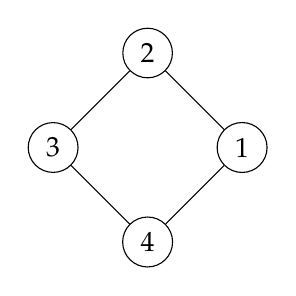
\begin{tikzpicture}[scale=0.6]
              % Define vertices
              \foreach \i in {1,2,3,4}
                \node[circle, draw, minimum size=0.3cm] (v\i) at ({90*(\i - 1)}:2cm) {\i};
              % Draw edges
              \foreach \i in {1,2,3}
                \draw (v\i) -- (v\the\numexpr\i+1\relax); % Connect consecutive vertices
              \draw (v4) -- (v1); % Connect the last and the first vertices to complete the cycle
        \end{tikzpicture}
        \caption{Graph $C_4$ corresponding to a rank 3 graphic matroid}
    \end{figure}
\end{frame}

\begin{frame}{History}
    \begin{itemize}
        \item 30 years ago, Mihail and Vazirani conjectured that the bases exchange walk mixes in polynomial time. 
        \item Polynomial mixing time corresponds to being able to count bases in polynomial time (Approximate sampling and approximate counting are equivalent in this scenario \cite[JVV86]{JVV86}).  
        \item Barvinok and Samorodnitsky designed a randomized algorithm that gives a $\log(n)^r$ approx. factor for a matroid with $n$ elements and rank $r$ \cite[BS07]{BS07}. 
        \item In Log-concave polynoimals I, Gharan et al. give a deterministic algorithm that returns an $e^r$ approximation factor.\cite[AKOV18]{AKOV18}
        \item In this paper, Gharan et al. give a randomized algorithm yielding a $1 \pm \ve$ approximation factor in polynomial time.
    \end{itemize}
\end{frame}


\begin{frame}{Main theorem}
    \begin{theorem}[1.1]
        Let $\mu: 2^{[n]} \to \R_{\geq 0}$ be a $d$-homogeneous strongly log concave probability distribution. If $P_\mu$ denotes the transition probability matrix of $M_\mu$ and $X(k)$ denotes the set of size-$k$ subsets of $[n]$ which are contained in some element of $\supp(\mu)$, then for every $0 \leq k \leq d-1$, $P_\mu$ has at most $|X(k)| \leq {n \choose k}$ eigenvalues of value $> 1 - \frac{k+1}d$. In particular, $M_\mu$ has spectral gap at least $1/d$, and if $\tau \in \supp(\mu)$ and $0 < \ve < 1$, the total variation mixing time of the Markov chain $M_\mu$ started at $\tau$ is at most $t_\tau(\ve) \leq d\log(\frac{1}{\ve\mu(\tau)})$.
    \end{theorem}
\end{frame}

\section{Preliminaries}
\subsection{Simplicial Complexes}
\begin{frame}{Simplicial Complexes}
\begin{definition}
    \begin{itemize}
        \item A set $X \subseteq 2^{[n]}$ is called a simplicial complex if whenever $\sigma \in X$ and $\tau \subset \sigma$, we have $\tau \in X$.
        \item Elements of $X$ are called faces, and the dimension of a face $\tau \in X$ is defined as $\dim(\tau) = |\tau|$.
        \item A face of dimension 1 is called a \textit{vertex}, and a face of dimension 2 is called an \textit{edge}.
        \item Define $X(k) = \Set{\tau \in X \mid \dim(\tau) = k}$ to be the collection of degree-$k$ faces of $X$.
    \end{itemize}
\end{definition}
\end{frame}

\begin{frame}{Examples}
    Any (undirected) graph $G = (V, E)$ is an example of a simplicial complex. 
    \begin{figure}[H]
        \centering
        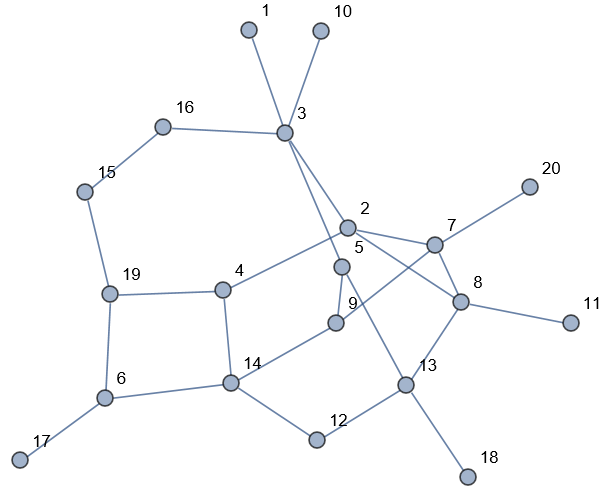
\includegraphics[width=0.6\textwidth]{imgs/RandomGraph.png}
        \caption{Example  of a simplicial complex}
        \label{fig:enter-label}
    \end{figure}
\end{frame}

\begin{frame}{Examples (contd.)}
    \begin{figure}[H]
        \centering
        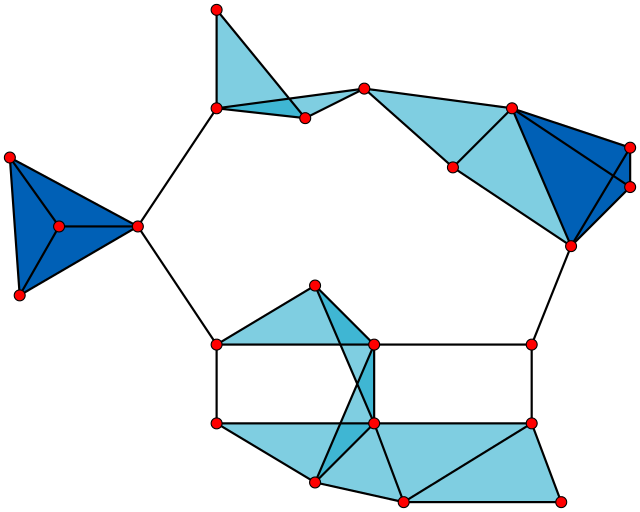
\includegraphics[width  = 0.7\textwidth]{imgs/Simplicial-Complex-Example.png}
        \caption{Example of a simplicial complex}
        \label{fig:enter-label}
    \end{figure}
\end{frame}

\begin{frame}{Definitions contd.}
    \small\begin{itemize}
        \item A simplicial complex $X$ is pure if all maximal (w.r.t. inclusion) faces have the same dimension. 
        \item The link of a face $\tau \in X$ is defined by $X_\tau = \Set{\sigma \setminus \tau \mid \sigma \in X, \; \tau \subset \sigma}$. Importantly, if $X$ is pure of dimension $d$ and $\tau \in X(k)$, then $X_\tau$ is pure of dimension $d-k$.
        \item Can equip a weight function $w: X \to \R_{> 0}$  to $X$ by assigning a positive weight to each face of $X$. Say a weight function $w: X \to \R_{> 0}$ is balanced if for any $\tau \in X$, $$w(\tau) = \sum_{\substack{\sigma \in X(k+1) \\ \tau \subset \sigma}} w(\sigma)$$
        \item Notice that we can equip $X$ with a (balanced) weight function by assigning its maximal faces weights and then assigning weights to the rest of the faces inductively.
    \end{itemize}
\end{frame}

\begin{frame}{Weights contd.}
\begin{itemize}
    \item Any (balanced) weight function on $X$ induces a weighted graph on the vertices of $X$ as follows: the 1-skeleton of $X$ is the (weighted) graph $G = (X(1), X(2), w)$ where $w$ has been restricted from $X$ to $X(2)$. In this case $w(v)$ for $v \in X(1)$ is the weighted degree of $v$.
\end{itemize}
\end{frame}

\begin{frame}{$d$-homogeneous polynomials}

    A polynomial $p \in \R[x_1, \ldots, x_n]$ is $d$-homogeneous if $p(\lambda x_1, \ldots, \lambda x_n) = \lambda^dp(x_1, \ldots, x_n)$ for every $\lambda \in \R$. Notice in this case that,
    \begin{align*}
        \sum_{k=1}^n x_k \partial_k p(x) = d \cdot p(x)
    \end{align*}

    Example. Consider $p(x, y, z) = xyz^2 + x^2yz$. Then,
    \begin{align*}
        \sum_{k=1}^3 x_k \partial_k p(x) &= (xyz^2 + 2x^2yz) + (xyz^2 + x^2yz) + (2xyz^2 + x^2yz) \\ &= 4xyz^2 + 4x^2yz
    \end{align*}
\end{frame}

\begin{frame}{Constructing Simplicial Complexes from Polynomials}
    From a $d$-homogeneous $p \in \R_{\geq 0}[x_1, \ldots, x_n]$ $p(x) = \sum_S c_Sx^S$, can construct a (weighted) simplicial complex $X^p$ by doing the following: include a $d$-dimensional face $S$ with weight $w(S) = c_S$ and include all subsets of these maximal faces inductively.
\end{frame}


\begin{frame}{Visuals}
    This polynomial yields the above (weighted) simplex where each tetrahedral face has weight 1: \begin{align*}
        p(x_1, \ldots, x_7) = x_1x_2x_3x_4 + x_3x_5x_6x_7
    \end{align*}
    \begin{figure}
        \centering
        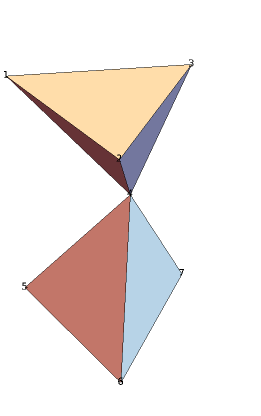
\includegraphics[angle=90, width=0.7\textwidth]{imgs/simplex.png}
        \caption{Two Tetrahedrons Glued Together}
        \label{fig:enter-label}
    \end{figure}
\end{frame}

\begin{frame}{Roadmap}
    \begin{figure}[H]
        \centering
        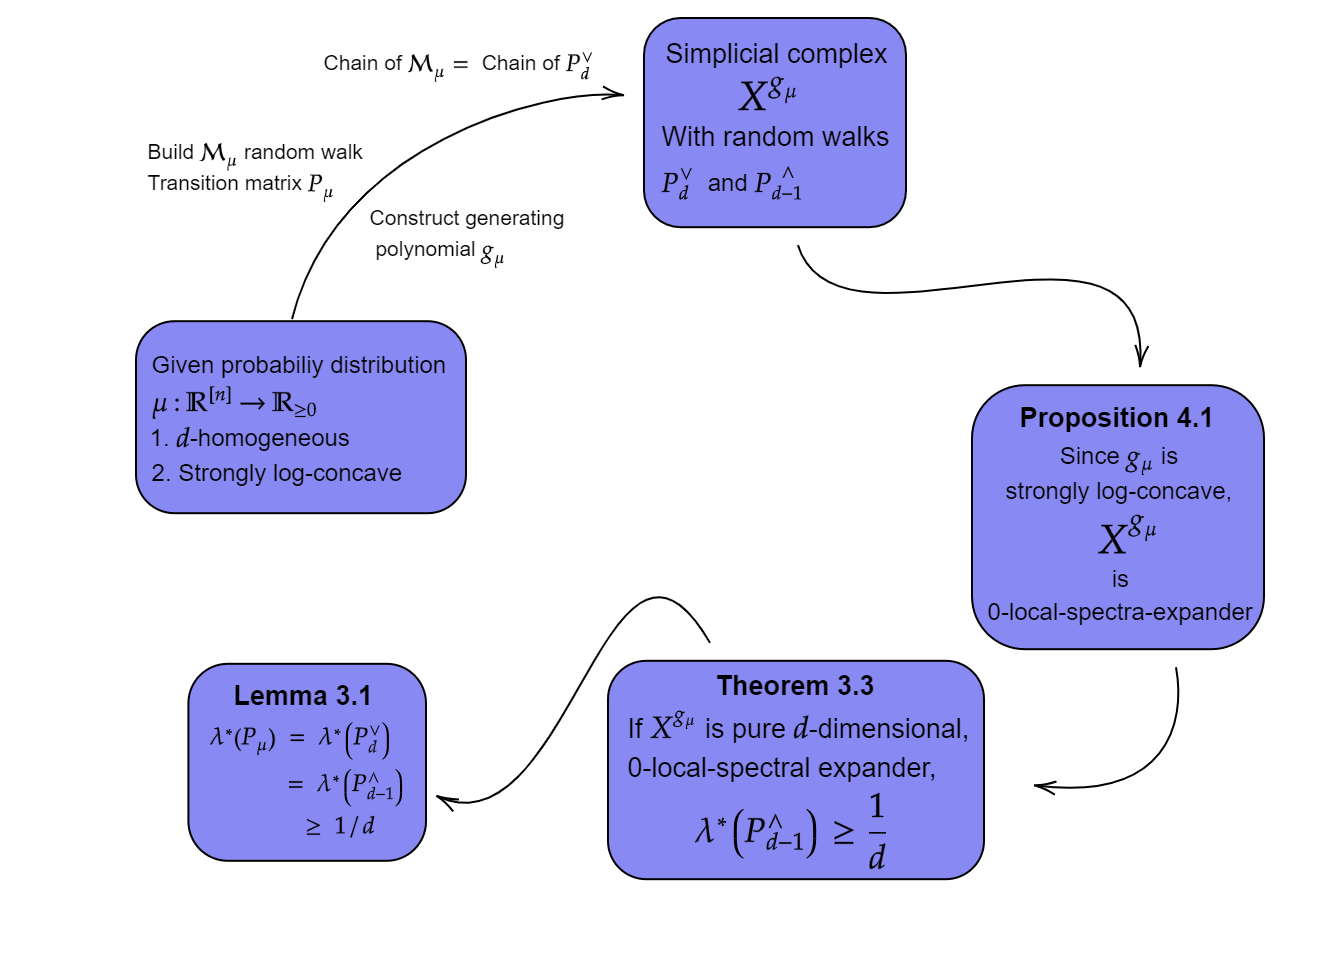
\includegraphics[width  = 0.8\textwidth]{imgs/diagram-20231214 (1).png}
        \caption{Roadmap}
        \label{fig:enter-label}
    \end{figure}
\end{frame}

\subsection{Log-concave polynomials}
\begin{frame}{Log-concave polynomial identities}
    \begin{definition}
    A polynomial $p \in \R_{\geq 0}[x_1, \ldots, x_n]$ is log-concave if $\log p$ is concave, equivalently if \begin{align*}
        \nabla^2 \log p = \frac{p \cdot (\nabla p)^2 - (\nabla p)(\nabla p)^T}{p^2}
    \end{align*}
    is NSD. For convience, define $p(x) \equiv 0$ to be log-concave.
    \end{definition}
\end{frame}

\begin{frame}{Log-concave properties contd.}
    \begin{itemize}
        \item By Cauchy's interlacing theorem, if $p$ is log-concave then $p \cdot (\nabla^2 p)$ has at most one positive eigenvalue at any $x \in \R^n_{> 0}$. 
        
        \item Since $p$ has nonnegative coefficients, log-concavity is equivalent to $\nabla^2 p \preceq \frac{(\nabla p)(\nabla p)^T}{p}$, so in this case $\nabla^2 p$ has at most 1 one positive eigenvalue.

        \item Turns out converse is true too: if $p$ is a degree $d$-homogeneous polynomial in $\R[x_1, \ldots, x_n]$, and $(\nabla^2 p)(x)$ has at most one positive eigenvalue for all $x \in \R^n_{>0}$, then $p$ is log-concave.

        \begin{definition} A polynomial $p \in \R[x_1, \ldots, x_n]$ is strongly log concave if for all $k \geq 0$ and all $\alpha \in [n]^k$, we have $\partial^{\alpha} p$ is log-concave (i.e., all sequences of partials are log-concave). \end{definition}
    \end{itemize}
\end{frame}


\subsection{Markov Chains and Random Walks}
\begin{frame}{Markov Chains and Random Walks}
    \begin{itemize}
        \item A Markov Chain is a triple $(\Omega, P, \pi)$ where $\Omega$ denotes a finite state space, $P \in \R^{\Omega \times \Omega}_{\geq 0}$ is a transition probability matrix. That is, \begin{align*}
            P(i,j) = P_{ij} = \mathbb{P}(X_{t+1} = j \hspace{2pt} \mid X_t = i)
        \end{align*} 
        It follows that the matrix is stochastic, such that $P \hspace{2pt} \mathbf{1} = \mathbf{1}$. 
        Finally, $\pi \in \R_{\geq 0}^\Omega$ denotes the stationary distribution of the chain ($\pi P = \pi$).
        \item The Markov Chain $(\Omega, P, \pi)$ is reversible if \begin{align*}
            \pi(\tau)P(\tau, \sigma) = \pi(\sigma)P(\sigma, \tau)
        \end{align*}
        for all $\tau, \sigma \in \Omega$.
    \end{itemize}
\end{frame}

\begin{frame}{Markov Chains and Random Walks continued}
\begin{itemize}
    \item For any reversible Markov chain ($\Omega$, $P$, $\pi$), the largest eigenvalue of $P$ is 1 (Perron-Fröbenius Theorem). We let $\lambda^*(P) = \max\{|\lambda_2|, |\lambda_n|\}$. The \textit{spectral gap} of the Markov chain is $1-\lambda^*(P)$.
    \begin{theorem}[2.9, (DS)]
    For any reversible irreducible Markov chain $(\Omega, P, \pi)$, $\epsilon > 0$, and any starting state
    \begin{align*}
        t_\tau(\epsilon) \leq \frac{1}{1-\lambda^*(P)}\cdot \log \left(\frac{1}{\epsilon \pi(\tau)}\right)
    \end{align*}
    where
    \begin{align*}
        t_\tau(\epsilon) = \min \Set{t \in \N \mid \norm{P^t(\tau, \cdot) - \pi}_1\leq \epsilon}
    \end{align*}
    \end{theorem}
\end{itemize}
\end{frame}

\section{Walks on Simplicial Complexes}
\subsection{Upper and lower walks}
\begin{frame}{Setting the stage}
\begin{itemize}
    \item Consider a pure $d$-dimensional complex $X$ with a balanced weight function $w : X \to \R_{>0}$.
    \item Going to define a bipartite graph $G_k$ with one side $X(k)$ and the other side $X(k+1)$. Connect $\tau \in X(k)$ to $\sigma \in X(k+1)$ with an edge of weight $w(\sigma)$ iff $\tau \subset \sigma$. Consider simple random walk on $G_k$: choose a neighbor proportional to the weight of the edge connecting the two vertices. 
\end{itemize}
\end{frame}

\begin{frame}{Examples}
    \begin{itemize}
        \item One on $X(k)$ called $P^\wedge_k$, where given $\tau \in X(k)$ you take two steps of the walk in $G_k$ to transition to the next $k$-face w.r.t. the $P^\wedge_k$ matrix.

        \item One on $X(k+1)$ called $P^\vee_{k+1}$, where given $\sigma \in X(k+1)$ you take two steps to transition to the next $k+1$ face w.r.t. $P^\vee_{k+1}$.
    \end{itemize}
    \begin{figure}[H]
    \centering
    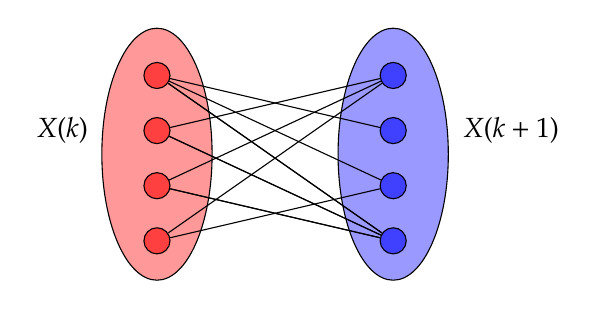
\begin{tikzpicture}
        \draw[fill = red!40] (0,1.8) ellipse (0.7cm and 1.6cm) node[] {};
        \draw[fill = blue!40] (3,1.8) ellipse (0.7cm and 1.6cm) node[] {};
        \foreach \i in {1, 2, 3, 4}{
            \node[circle, draw, fill = red!75] (L\i) at (0, 0.7*\i){};
            \node[circle, draw, fill = blue!75] (R\i) at (3, 0.7*\i){};
        }
        \draw (L1) -- (R2);
        \draw (L2) -- (R1);
        \draw (L3) -- (R1);
        \draw (L4) -- (R3);
        \draw (L4) -- (R1);
        \draw (L4) -- (R2);
        
        \draw (L3) -- (R4);
        \draw (L2) -- (R4);
        \draw (L1) -- (R4);

        \draw (L2) -- (R1);
        \draw (L3) -- (R1);
        \draw (L4) -- (R1);
        \node at (-1.2, 2.1) {$X(k)$};
        \node at (4.5, 2.1)  {$X(k+1)$};
    \end{tikzpicture}
    \caption{Bipartite graph $G_k$}
    \end{figure}
\end{frame}

% \begin{frame}{Probabilities}
% \begin{itemize}
%     \item Given a face $\tau \in X(k)$, among all $\sigma \in X(k+1)$ containing $\tau$ choose one proportional to $w(\sigma)$. Then delete one of the $|\sigma| = k+1$ elements of $\sigma$ u.a.r. to obtain a new state $\tau'$. Then the probability of transition to $\tau'$ is equal to choosing $\sigma = \tau \cup \tau'$ in the first step, which is equal to $$\frac{w(\tau \cup \tau')}{w(\tau)} = \frac{w(\sigma)}{\sum_{\substack{\psi \in X(k+1) \\ \tau \subset \psi}} w(\psi)},$$
%     since $w$ is balanced, times the probability of choosing $\tau'$ from $\sigma$, which is $\frac{1}{k+1}$. Analysis for $P^\vee_k$ is similar, so get:
% \end{itemize}    
% \end{frame}

\begin{frame}{Values of the transition matrix}
    \small\begin{align*}
        P_k^{\wedge}(\tau, \tau') = 
        \begin{cases}
            \frac{1}{k+1} & \text{if }  \tau = \tau'  \\
            \frac{w(\tau \cup \tau')}{(k+1)w(\tau)} &  \text{if } \tau \cup \tau'  = X(k+1) \\
            0,  &  \text{ otherwise}
        \end{cases} 
    \end{align*}
    \begin{align*}
        P_{k+1}^{\vee}(\sigma, \sigma') = 
        \begin{cases}
            \sum_{\tau \in X(k);  \hspace{2pt} \tau \subset \sigma} \frac{w(\sigma)}{(k+1)w(\tau)} & \text{if }  \sigma = \sigma'  \\
                    \frac{w(\sigma')}{(k+1)w(\sigma \cap \sigma')} &  \text{if } \sigma \cap \sigma'  = X(k) \\
            0,  &  \text{ otherwise}
        \end{cases} 
    \end{align*}
    Note that both random walks are reversible with the same stationary distribution: \begin{align*}
        w(\tau)P^\wedge_k(\tau, \tau') = w(\tau')P^\wedge_k(\tau', \tau) \quad \text{ and } \quad w(\sigma)P^\vee_{k+1}(\sigma, \sigma') = w(\sigma')P^\vee_{k+1}(\sigma', \sigma)
    \end{align*}
\end{frame}

\subsection{0-local-spectral-expanders}

\subsection{$\lambda^*(P_d^{\wedge})  = \lambda^*(P_{d-1}^{\vee})$}
\begin{frame}{Proving $\lambda^*(P_d^{\wedge})  = \lambda^*(P_{d-1}^{\vee})$}
\begin{fact}[Useful]
    \vspace{2pt}
    Let \( A \in \mathbb{R}^{n \times k} \) and \( B \in \mathbb{R}^{k \times n} \) be arbitrary matrices. Then, non-zero eigenvalues of \( AB \) are equal to non-zero eigenvalues of \( BA \) with the same multiplicity.
\end{fact}

\begin{lemma}[3.1]
    \vspace{2pt}
    For any $1 \leq k \leq d$, $P^{\wedge}_k$ and $P_{k+1}^{\vee}$ are stochastic, self-adjoint w.r.t. the $\omega$-induced inner product, $PSD$, and have the same (with multiplicity) non-zero eigenvalues.
\end{lemma}
\end{frame}

\begin{frame}{Proving $\lambda^*(P_d^{\wedge})  = \lambda^*(P_{d-1}^{\vee})$}
    \begin{proof}
        Since $G_k$ is bipartite, we may write the transition of the random walk on $G_k$ as \begin{align*}
            P_k = \begin{bmatrix}
                0  & P_k^{\downarrow} \\
                P_k^{\uparrow} & 0
            \end{bmatrix}
        \end{align*}
        Note that $P_k^{\uparrow}$ and $P_k^{\downarrow}$ are stochastic matrices. Then we see that \begin{align*}
            P_k^2 = \begin{bmatrix}
                P_k^{\downarrow}P_k^{\uparrow}  &  \\
                &  P_k^{\uparrow}P_k^{\downarrow}
            \end{bmatrix}
        \end{align*}
        It is easy to see $P_k^2$ is PSD and stochastic. But now we note that $P_k^\wedge =  P_k^{\downarrow}P_k^{\uparrow}$ and $P_{k+1}^\vee = P_k^{\uparrow}P_k^{\downarrow}$ and we're done.  
    \end{proof}
\end{frame}

\begin{frame}{Looking at $P^\wedge_1$}
    \begin{itemize}
        \item  \( P^{\wedge}_1 \) is the transition probability matrix of the simple \((1/2)\)-lazy random walk on the weighted 1-skeleton of \( X \) where the weight of each edge \( e \in X(2) \) is \( w(e) \).
        \item Also consider the non-lazy variant of this random walk, given by the transition matrix \( \widetilde{P}^{\wedge}_1= 2(P^{\wedge}_1 - I/2) \)
        \item Similarly, for any face \( \tau \in X(k) \), we define the upper random walk on the faces of the link \( X_{\tau} \). Specifically, let \( P^{\wedge}_{\tau,1} \) denote the transition matrix of the upper walk, as above, on the 1-dimensional faces of \( X_{\tau} \), and \( \widetilde{P}^{\wedge}_{\tau, 1} = 2(P^{\wedge}_{\tau, 1} - I/2) \) be the transition matrix for the non-lazy version.
    \end{itemize}
     
    \begin{definition}[Local Spectral Expanders, KO18]
          For \( \lambda > 0 \), a pure \( d \)-dimensional weighted complex \( (X, w) \) is a \( \lambda \)-local-spectral-expander if for every \( 0 \leq k < d - 1 \), and for every \( \tau \in X(k) \), we have \( \lambda_2(\widetilde{P}^{\wedge}_{\tau, 1}) \leq \lambda \).
    \end{definition}
\end{frame}

\begin{frame}{Theorem 3.3}
    \begin{theorem} 
        \vspace{2pt}
        Let $(X, w)$ be a pure $d$-dimensional weighted 0-local spectral expander and let $0 \leq k < d$. Then for all $-1 \leq i \leq k$, $P_k^\wedge$ has at most $|X(i)| \leq {n \choose i}$ eigenvalues of value $> 1 - \frac{i+1}{k+1}$, where (by convention) $X(-1) = \emptyset$ and ${n \choose -1} = 0$. In particular, the second largest eigenvalue of $P_k^\wedge$ is at most $\frac{k}{k+1}$. 
    \end{theorem}

    \begin{lemma}
        \vspace{2pt}
        $P_k^\wedge \preceq \frac{k}{k+1} P_k^\vee + \frac{1}{k+1}I$ for all $0 \leq k < d$.
    \end{lemma}
\end{frame}

\iffalse
\begin{frame}{Proof of Theorem 3.3}
    The case $k = 0$ is trivial. When $k = 1$, $P_1^\wedge = \frac12(\tilde{P}_1^\wedge + I)$. Since $(X, w)$ is a 0-local spectral expander, $\tilde P_1^\wedge$ has exactly one positive eigenvalue with value 1. So, $P_1^\wedge$ has eignevalue 1 with multiplicity 1. All the others are less than or equal to $1/2$ and there are $|X(1)| - 1$ many. 

    Assume the claim holds for some $d-1 > k \geq 0$. By lemma, $P_{k+1}^\vee$ has the same non-zero eigenvalues as $P_k^\wedge$. By lemma, 
    \begin{align*}
        P^\wedge_{k+1} \preceq \frac{k+1}{k+2} P_{k+1}^\vee + \frac{1}{k+2}I
    \end{align*}
    By induction $P_k^\wedge$ has at most $|X(i)|$ eigenvalues $> 1 - \frac{i+1}{k+1}$. So, $P^\wedge_{k+1}$ has at most $|X(i)|$ eigenvalues $>\frac{k+1}{k+2}(1-\frac{i+1}{k+1}) + \frac{1}{k+2} = 1 - \frac{i+1}{k+2}$. For $i = k+1$, trivial since $P^\wedge_{k+1} \in \R^{|X(k+1)| \times |X(k+1)|}$.
\end{frame}
\fi

\section{From log-concavity to Local Spectral Expanders}
\subsection{Strong Log-Concavity implies 0-local-spectral-expander}
\begin{frame}{From log-concavity to Local Spectral Expanders}
\begin{theorem}[Proposition 4.1]
    \vspace{2pt}
    Let \( p \in \mathbb{R}[x_1, \ldots, x_n] \) be a multiaffine homogeneous polynomial with nonnegative coefficients. If \( p \) is strongly log-concave, then \( (X^p, w) \) is a \( 0 \)-local-spectral-expander, where \( w(S) = c_S \) for every maximal face \( S \in X^p \)
\end{theorem}

\begin{itemize}
    \item Let $p_\tau  = \left( \prod_{i \in \tau} \partial_i\right)p$
\end{itemize}
\begin{lemma}[4.2]
    For any $0 \leq k \leq d$, and any simplex $\tau \in X^p(k)$, $w(\tau) = (d-k)!p_\tau(\mathbf 1)$. 
\end{lemma}
\end{frame}

\begin{frame}{From log-concavity to Local Spectral Expanders}
    \footnotesize\begin{lemma}[Lemma  4.2]
        For any $0 \leq k \leq d$, and any simplex $\tau \in X^p(k)$, $w(\tau) = (d-k)!p_\tau(\mathbf 1)$. 
    \end{lemma}
    \begin{proof}[Proof of Lemma.]
    Induction on $d-k$. If $\dim(\tau) = d$, then $p_\tau = c_\tau$, and done. So suppose statement holds for $\sigma \in X^p(k+1)$ and fix simplex $\tau \in X^p(k)$. Then,
    \begin{align*}
        w(\tau) = \sum_{\substack{\sigma \in X^p(k+1) \\ \tau \subset \sigma}} w(\sigma) = \sum_{i \in X^p_\tau(1)} w(\tau \cup \Set{i})
    \end{align*}

    Since $\partial_i p_\tau = 0$ for $i \not \in X_\tau^p(1)$, we have
    \begin{align*}
        w(\tau) = (d-k-1)!\sum_{i \in X^p_\tau(1)} p_{\tau \cup \Set{i}}(\mathbf 1) = (d-k-1)!\sum_{i=1}^n \partial_i p_\tau(\mathbf 1) = (d-k)! p_\tau(\mathbf 1)
    \end{align*}
    Where the last equality holds by Euler's identity.
    \end{proof}
\end{frame}

\begin{frame}{Proof of Proposition 4.1}
    Since $p$ is strongly log-concave, $\nabla^2 p(\mathbf 1)$ has at most one positive eigenvalue. Let
    \begin{align*}
        \tilde \nabla^2 p = \frac{1}{d-k-1} (\mathrm{diag}(\nabla p))^{-1} \nabla^2 p(\mathbf 1)
    \end{align*}
    Claim: $\tilde \nabla^2 p = \tilde P^\wedge_{\tau, 1}$. Note that 
    \begin{align*}
        \tilde P^\wedge_{\tau, 1}(i, j) = \frac{w_\tau(\Set{i, j})}{w_\tau(\Set{i})} = \frac{w(\tau \cup \Set{i, j})}{w(\tau \cup \Set{i})}
    \end{align*}
    While,
    \begin{align*}
        (\tilde \nabla^2 p)(i,j) = \frac{(\partial_i \partial_j p)(\mathbf 1)}{(d-k-1)(\partial_i p)(\mathbf 1)}
    \end{align*}
    By lemma, equal.
\end{frame}

\begin{frame}{Proof contd.}
    Since $p$ has nonnegative coefficients, the vector $(\nabla p)(\mathbf 1)$ has nonnegative entries which implies $\mathrm {diag}(\nabla p)(\mathbf 1) \succeq 0$. Fact: if $B \succeq 0$ and $A$ has (at most) $k$ positive eigenvalues then $BA$ has at most $k$ positive eigenvalues. Since $(\nabla^2 p)(\mathbf 1)$ has at most 1 positive eigenvalue, $\tilde \nabla^2 p$ has at most 1 positive eigenvalue by the fact. Thus, $\tilde \nabla^2 p = \tilde P^\wedge_{\tau, 1}$ has at most one positive eigenvalue, so $\lambda_2(\tilde P^\wedge_{\tau, 1}) \leq 0$. $\hfill \qedsymbol$
\end{frame}

\section{Putting everything together: Proof of Theorem 1.1}

\begin{frame}{Generating polynomial of $\mu$ and $\mathcal{M}_\mu$}
\begin{itemize}
    \item Let $\mu: 2^{[n]} \to \R_{\geq 0}$ be a probability distribution. Assing a multiaffine polynomial with variables $x_1 \ldots, x_n$ to $\mu$:
    \begin{align*}
        g_\mu(x) = \sum_{S\subset [n]} \mu(S) \cdot \prod_{i \in S} x_i
    \end{align*}
    \item Say $\mu$ is $d$-homogeneous if $g_\mu$ is $d$-homogeneous, and (strongly) log-concave if $g_\mu$ is. 
    \item We can define a random walk $\mathcal{M}_\mu$ by the following: We take the state space of $M_\mu$ to be the support of $\mu$, namely $\text{supp}(\mu) = \{S \subseteq [n] \,|\, \mu(S) \neq 0\}$. For $\tau \in \text{supp}(\mu)$, first we drop an element $i \in \tau$, chosen uniformly at random from $\tau$. Then, among all sets $\sigma \supseteq \tau \setminus \{i\}$ in the support of $\mu$, we choose one with probability proportional to $\mu(\sigma)$.
 
\end{itemize}
\end{frame}

\begin{frame}{Proof of Theorem 1.1}
    \footnotesize\begin{theorem}[1.1]
        Let $\mu: 2^{[n]} \to \R_{\geq 0}$ be a $d$-homogeneous strongly log concave probability distribution. If $P_\mu$ denotes the transition probability matrix of $M_\mu$ and $X(k)$ denotes the set of size-$k$ subsets of $[n]$ which are contained in some element of $\supp(\mu)$, then for every $0 \leq k \leq d-1$, $P_\mu$ has at most $|X(k)| \leq {n \choose k}$ eigenvalues of value $> 1 - \frac{k+1}d$. In particular, $M_\mu$ has spectral gap at least $1/d$, and if $\tau \in \supp(\mu)$ and $0 < \ve < 1$, the total variation mixing time of the Markov chain $M_\mu$ started at $\tau$ is at most $t_\tau(\ve) \leq d\log(\frac{1}{\ve\mu(t)})$.
    \end{theorem}
    \begin{proof}
         Let \( \mu \) be a \( d \)-homogeneous strongly log-concave distribution, and let \( P_{\mu} \) be the transition probability matrix of the chain \( M_{\mu} \). By Theorem 2.9, it is enough to show that \( \lambda^*(P_{\mu}) \leq 1 - \frac{1}{d} \). Observe that the chain \( M_{\mu} \) is exactly the same as the chain \( P^{\vee}_d \) for the simplicial complex \( X^{g_{\mu}} \) defined above. Therefore, \( \lambda^*(P_{\mu}) = \lambda^*(P^{\vee}_d) = \lambda^*(P^{\wedge}_{d-1}) \), where the last equality follows by Lemma 3.1. Since \( g_{\mu} \) is strongly log-concave, by Proposition 4.1, \( X^{g_{\mu}} \) is a \( 0 \)-local-spectral-expander. Therefore, by Theorem 3.3, \( \lambda^*(P^{\wedge}_{d-1}) \leq 1 - \frac{1}{(d-1) + 1} = 1 - \frac{1}{d} \).
    \end{proof}       
\end{frame}

\begin{frame}{Roadmap}
    \begin{figure}[H]
        \centering
        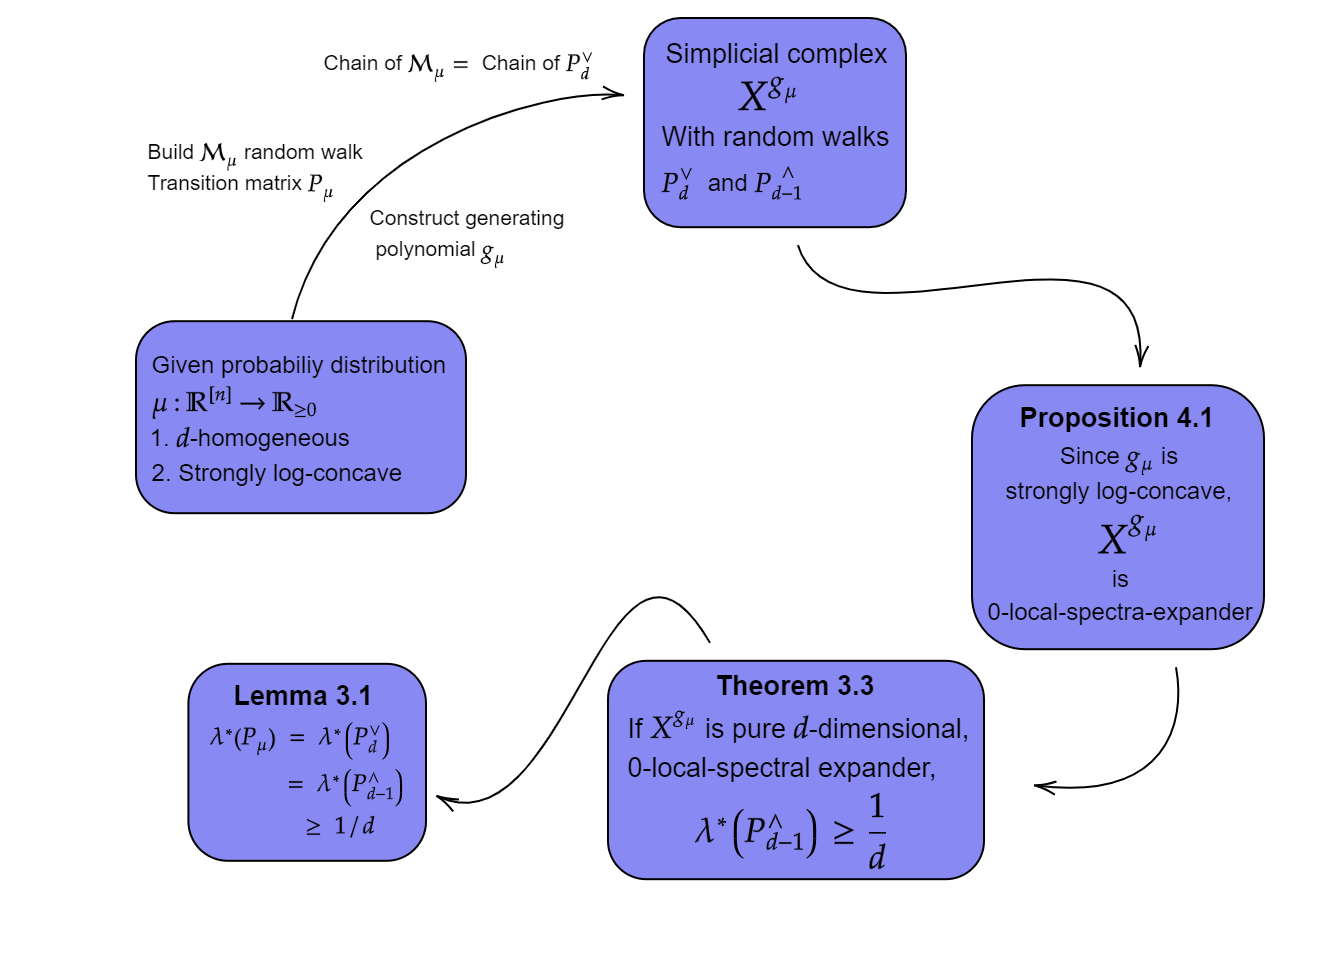
\includegraphics[width  = 0.8\textwidth]{imgs/diagram-20231214 (1).png}
        \caption{Roadmap}
        \label{fig:enter-label}
    \end{figure}
\end{frame}


\section[References]{References}
\begin{frame}{References}
\footnotesize\begin{thebibliography}{9}
    \bibitem{AKOV19}
    Anari, N., Liu, K., Gharan, S. O., Vinzant, C. (2019, June). \emph{Log-concave polynomials II: High-dimensional walks and an FPRAS for counting bases of a matroid}. In Proceedings of the  51st Annual ACM SIGACT Symposium on Theory of Computing (pp. 1-16).
    \bibitem{JVV86}  
    Mark Jerrum, Leslie Valiant, and Vijay Vazirani. “Random Generation of Combinatorial Structures from a Uniform Distribution”. In: Theoretical Computer Science 43 (1986), pp. 169–188.
    \bibitem{AKOV18}
    Nima Anari, Shayan Oveis Gharan, and Cynthia Vinzant. “Log-concave polynomials, entropy, and a deterministic approximation algorithm for counting bases of matroids”. In: \textit{FOCS}. to appear. 2018.
    \bibitem{BS07}
    Alexander Barvinok and Alex Samorodnitsky. “Random weighting, asymptotic counting, and inverse isoperimetry”. In: Israel Journal of Mathematics 158.1 (Mar. 2007), pp. 159–191. issn: 1565-8511.
\end{thebibliography}
\end{frame}
\end{document}
